\documentclass{beamer}

\usetheme{Boadilla}
%\usetheme{Warsaw}
%\setbeamercovered{transparent}
\beamertemplatetransparentcoveredhigh
\usepackage[portuges]{babel}
\usepackage[latin1]{inputenc}
\usepackage{ulem}
\usepackage{lmodern}
\usepackage[T1]{fontenc}

\newcommand{\eng}[1]{\textsl{#1}}
\newcommand{\cod}[1]{\texttt{#1}}


\title[9002 --- Aula 09]{9002 --- Aula 09\\
   Algoritmos e Programa��o de Computadores}

\author[IEng - UFMT]{Instituto de Engenharia -- UFMT}

\institute[2014/2]{Segundo Semestre de 2014}

\date{14 de outubro de 2014}


\begin{document}

\begin{frame}[plain]
  \titlepage
\end{frame}

\begin{frame}
  \frametitle{Roteiro}
  \tableofcontents
\end{frame}

\section{Comando for}


\begin{frame}[fragile]
    \frametitle{Comando de repeti��o t�pico}

    \begin{exampleblock}{}
    \cod{\noindent
      int i; \\
      \alert<2>{i = 0}; \\
      while (\alert<3>{i < 100}) \{ \\
        \hspace*{1cm}printf("\%d", i);\\
        \hspace*{1cm}\alert<4>{i = i + 1};\\
      \}
    }
    \end{exampleblock}

    Partes t�picas:
    \begin{itemize}
      \item<2-> \alert<2>{\textbf{In�cio}}: Inicializa as vari�veis (normalmente �ndices e acumuladores).
      \item<3-> \alert<3>{\textbf{Condi��o}}: Valor booleano que indica a condi��o para executar.
      \item<4-> \alert<4>{\textbf{Passo}}: Atualiza as vari�veis (normalmente os �ndices).
    \end{itemize}
\end{frame}

\begin{frame}[fragile]
    \frametitle{Comando for}

    \begin{block}{Sintaxe do \cod{for}}
\begin{semiverbatim}
for (\alert{inicio} ; \alert{condicao} ; \alert{passo}) \{
    comandos;
\}
\end{semiverbatim}     
    \end{block}

    \only<1>{
    Partes:
    \begin{itemize}
      \item \textbf{In�cio}: Um ou mais comandos de atribui��o separadas por \alert{,}
      \item \textbf{Condi��o}: Valor booleano que indica a condi��o para executar
      \item \textbf{Passo}: Um ou mais comandos de atribui��o separados por \alert{,}
    \end{itemize}
    }

    \only<2>{
  Funcionamento:
  \begin{itemize}
    \item \textbf{Passo 1}: Executa comandos em ``inicio''.
    \item \textbf{Passo 2}: Testa condi��o.\\
      \hspace*{1cm} Se condi��o for \alert{verdadeira}, vai para o Passo 3.\\
      \hspace*{1cm} Se condi��o for \alert{falsa}, continua o programa.
    \item \textbf{Passo 3}:\\
      \hspace*{1cm} \textbf{(a)} Executa comandos.\\
      \hspace*{1cm} \textbf{(b)} Executa comandos em ``passo''.\\
      \hspace*{1cm} \textbf{(c)} Volta ao Passo 2.
  \end{itemize}
  }
\end{frame}

\begin{frame}[fragile]
  \frametitle{Imprimindo os 100 primeiros n�meros inteiros}

  \begin{exampleblock}{}
\begin{verbatim}
int i;
for(i = 1; i<= 100; i=i+1){
    printf("\n %d",i);
}  \end{verbatim}
  \end{exampleblock}
\end{frame}

\begin{frame}[fragile]
  \frametitle{Imprimindo os $n$ primeiros n�meros inteiros}

  \begin{exampleblock}{}
\begin{verbatim}
int i, n;
scanf("%d",&n);
for(i=1; i<=n; i++){
    printf("\n %d",i);
}  \end{verbatim}
  \end{exampleblock}
\end{frame}

\begin{frame}[fragile]
  \frametitle{Imprimindo as $n$ primeiras pot�ncias de 2}

  \begin{exampleblock}{}
\begin{verbatim}
int i, n, pot;
pot = 2;
scanf("%d",&n);
for(i=1; i <= n; i++){
    printf("\n %d",pot);
    pot = pot *2;
}  \end{verbatim}
  \end{exampleblock}
\end{frame}

\begin{frame}
  \frametitle{N�o atirarei mais avi�es em aula}

  \begin{center}
    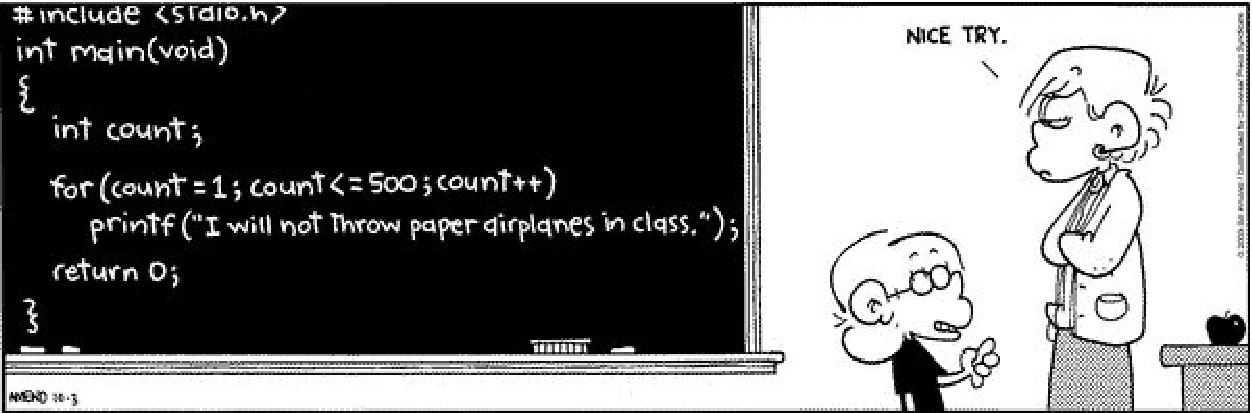
\includegraphics[width=11cm]{joke.pdf}
  \end{center}
\end{frame}

\section{Exerc\'icios}
\begin{frame}
  \frametitle{Exerc�cios}

  \begin{itemize}
  \item Fa�a um programa que l� dois n�meros inteiros $n$ e $a$ e imprime o resultado de $a^n$.
  
  \item Fa�a um programa que l� um n�mero n e imprime os valores entre 2 e n, que s�o divisores de n.
  
  \item Fa�a um programa que determina se um n�mero inteiro lido do teclado � primo ou composto.
  \end{itemize}
\end{frame}

\section{Nas Pr�ximas Aulas...}
\begin{frame}
  \frametitle{Nas Pr�ximas Aulas...}

  \begin{itemize}
  \item veremos exemplos de comandos de repeti\c{c}�o encaixados e resolveremos mais exerc�cios.
  
  \item FIM!!!
  \end{itemize}
\end{frame}


\end{document}

